\chapter{DASAR TEORI}
\par Bab ini menjelaskan dasar teori yang penulis gunakan sebagai landasan pengerjaan tugas akhir. Bab ini akan menjelaskan secara umum terkait istilah dan kakas bantu yang digunakan dalam pembuatan tugas akhir ini.

\section{Penelitian Sebelumnya}
\par Tugas akhir ini merupakan pengembangan lanjutan dari penelitian "Rancang Bangun Aplikasi Push Notification Terpusat". Penelitian tersebut menghasilkan aplikasi yang bernama Push Notification Terpusat. Aplikasi tersebut digunakan untuk mengirim \textit{push notification} ke perangkat pengguna di ITS.
\par Akan tetapi, aplikasi yang telah dibangun masih memiliki kelemahan dari sisi keandalan aplikasi. Hasil uji dapat dilihat pada Tabel \ref{t:hasil_uji_sebelum}.
\begin{longtable}{|p{1.5cm}|p{2cm}|p{2cm}|p{2.5cm}|}
	\caption{Hasil Uji Penelitian Sebelumnya \cite{application-thesis}} \label{t:hasil_uji_sebelum} \\ \hline
	\rowcolor{lightgray} Kode Uji & Jumlah Pengguna & Tingkat Keberhasilan & Rata-Rata \textit{Response Time} (detik) \\ \hline
	RT001 & 100 & 100\% & 0,334 \\ \hline
	RT002 & 500 & 100\% & 2,326 \\ \hline
	RT003 & 1000 & 100\% & 4,664 \\ \hline
	RT004 & 2000 & 80,7\% & 8,889 \\ \hline
	RT005 & 3000 & 63,8\% & 10,552 \\ \hline
\end{longtable}
\par Berdasarkan hasil uji, dapat disimpulkan bahwa aplikasi yang dibangun sebelumnya hanya dapat menangani maksimum seribu pengguna. Jumlah ini dianggap belum dapat memenuhi kebutuhan karena target pengguna aplikasi ini adalah mahasiswa, dosen, dan karyawan yang ada di ITS.
\par Oleh karena itu, pengembangan yang diterapkan pada tugas akhir ini akan berfokus untuk meningkatkan keandalan aplikasi, agar aplikasi dapat menangani hingga 100 ribu pengguna.

\section{Push Notification Terpusat}
\par Push Notification Terpusat merupakan aplikasi yang dibuat untuk memudahkan penyebaran informasi di lingkungan ITS sebagai pengganti media cetak. Aplikasi ini dapat mengirimkan push notification secara langsung atau terjadwal ke perangkat pengguna (Android dan iOS) \cite{application-thesis}. Arsitektur aplikasi saat ini dapat dilihat pada Gambar \ref{img:arsitektur-pnt_lama}.
\begin{figure}[H]
	\centering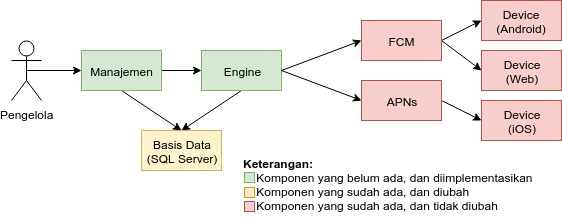
\includegraphics[width=0.8\textwidth]{bab2/img/arsitektur-push_notification_terpusat_lama.jpg}
	\caption{Arsitektur Push Notification Terpusat Saat Ini}
	\label{img:arsitektur-pnt_lama}
\end{figure}
\par Aplikasi terdiri dari 2 modul, yaitu manajemen dan \textit{engine}. Modul manajemen bertanggung jawab untuk menangani interaksi pengelola dengan sistem lewat halaman berbasis web, sementara modul \textit{engine} bertanggung jawab untuk mengirimkan \textit{push notification}.
\par Pengembangan yang dilakukan pada tugas akhir ini berfokus di keandalan pengiriman \textit{push notification}, sehingga hanya modul \textit{engine} saja yang akan mengalami perubahan. 

\section{iOS}
\par iOS adalah sistem operasi perangkat bergerak yang dikembangkan oleh Apple untuk perangkat iPhone, iPad, dan iPod \cite{ios-online}.
\par Pada tugas akhir ini, perangkat dengan sistem operasi iOS merupakan salah satu target penerima \textit{push notification} yang dikirim oleh Push Notification Terpusat.

\section{Android}
\par Android adalah sistem operasi perangkat bergerak yang dikembangkan oleh Google untuk ponsel, pakaian, tablet, televisi, dan kendaraan \cite{android-online}.
\par Pada tugas akhir ini, perangkat dengan sistem operasi Android merupakan salah satu target penerima \textit{push notification} yang dikirim oleh Push Notification Terpusat.

\section{Apple Push Notification Service}
\par Apple Push Notification Service atau APNs adalah layanan pengiriman notifikasi jarak jauh yang kuat, cepat dan sangat efisien, yang dapat digunakan oleh pengembang aplikasi untuk menyebarkan informasi ke perangkat iOS, watchOS, tvOS, dan macOS. Ukuran maksimum notifikasi yang dapat dikirim adalah 4 Kb, dan wajib menggunakan protokol TLS, dengan alur yang dapat dilihat pada Gambar \ref{img:apns-certificate} \cite{apns-online}.
\begin{figure}[H]
	\centering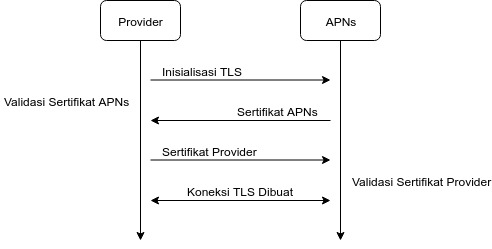
\includegraphics[width=0.7\textwidth]{bab2/img/activity-apns_certificate_connection.jpg}
	\caption{Alur Autentikasi APNs}
	\label{img:apns-certificate}
\end{figure}
\par Untuk dapat menerima dan mengontrol remote notification, aplikasi harus memenuhi syarat sebagai berikut.
\begin{enumerate}
	\item Mengaktifkan kemampuan push notifications dengan cara memindah switch posisi \textit{off} menjadi \textit{on} pada jendela \textit{Project editor} > \textit{Target} > \textit{Capabilities}.
	\item Melakukan registrasi aplikasi kepada APNs dengan cara menerima token yang bersifat unik untuk tiap perangkat yang berbeda.
	\item Sistem akan menampilkan perangkat ke aplikasi Anda dengan memanggil metode di delegasi aplikasi. Aplikasi mengirimkan token perangkat ke penyedia yang terkait dengan aplikasi.
\end{enumerate}
\par Contoh program yang digunakan untuk mengirim notifikasi ke perangkat iOS lewat layanan APNs dapat dilihat pada Kode Sumber \ref{json:contoh-apns}. Hasil notifikasi yang diterima oleh pengguna dapat dilihat pada Gambar \ref{img:contoh-hasil-apns}.
\lstinputlisting[label=json:contoh-apns, caption={Contoh Push Notification APNs}] {bab2/json/apns.json}
\begin{figure}[H]
	\centering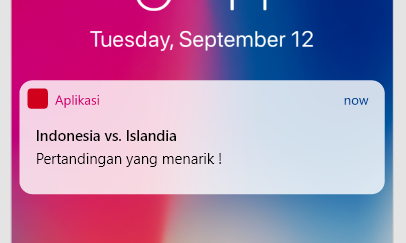
\includegraphics[width=0.5\textwidth]{bab2/img/apns.png}
	\caption{Pratinjau Notifikasi pada iOS}
	\label{img:contoh-hasil-apns}
\end{figure}
\par Pada tugas akhir ini, \textit{push notification} yang menargetkan perangkat iOS akan dikirim dengan menggunakan layanan Apple Push Notification Service.

\section{Firebase Cloud Messaging}
\par Firebase Cloud Messaging atau FCM adalah solusi pengiriman pesan lintas platform yang dapat diandalkan untuk mengirimkan pesan dan dapat digunakan tanpa biaya. FCM memiliki kemampuan sebagai berikut \cite{fcm-online}:
\begin{enumerate}
	\item Mengirimkan notifikasi atau pesan data
	\par Mengirim pesan notifikasi yang ditampilkan kepada pengguna. Atau mengirim pesan data dan menentukan sepenuhnya apa yang terjadi dalam kode aplikasi.
	\item Penargetan pesan serbaguna
	\par Mendistribusikan pesan ke aplikasi klien dengan salah satu dari tiga cara — ke satu perangkat, ke grup perangkat, atau ke perangkat yang berlangganan topik.
	\item Mengirim pesan dari aplikasi \textit{client}
	\par Mengirim notifikasi, chat, dan pesan lain dari perangkat ke server melalui saluran koneksi FCM yang andal dan hemat baterai.
\end{enumerate}
\par Untuk mengimplementasikan FCM, pengembang harus mengikuti langkah-langkah berikut:
\begin{enumerate}
	\item Menyiapkan FCM SDK
	\par Menyiapkan Firebase dan FCM pada aplikasi sesuai petunjuk penyiapan untuk \textit{platform} (Android atau Web).
	\item Mengembangkan aplikasi klien
	\par Menambahkan penanganan pesan, logika langganan topik, atau fitur opsional lain ke aplikasi \textit{client}. Selama pengembangan, dapat dilakukan pengujian untuk mengirim pesan dengan mudah menggunakan \textit{Firebase Console}.
	\item Mengembangkan server aplikasi
	\par Tentukan apakah pengembangan nantinya menggunakan Admin SDK atau salah satu server \textit{protocol} untuk membuat logika pengiriman, yaitu logika untuk mengautentikasi, membuat permintaan pengiriman, menangani respons, dan sebagainya.
\end{enumerate}
\par Contoh program yang digunakan untuk mengirim notifikasi ke perangkat Android lewat layanan FCM dapat dilihat pada Kode Sumber \ref{json:contoh-fcm}. Hasil notifikasi yang diterima oleh pengguna dapat dilihat pada Gambar \ref{img:contoh-hasil-fcm}.
\lstinputlisting[label=json:contoh-fcm, caption={Contoh Push Notification FCM}] {bab2/json/fcm.json}
\begin{figure}[H]
	\centering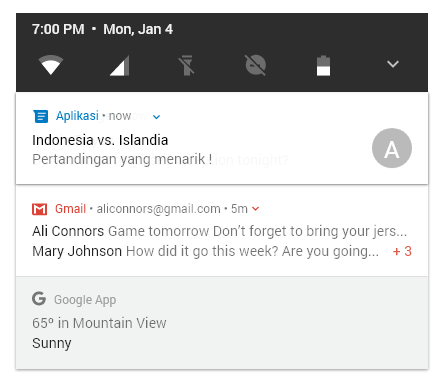
\includegraphics[width=0.5\textwidth]{bab2/img/fcm.png}
	\caption{Pratinjau Notifikasi pada Android}
	\label{img:contoh-hasil-fcm}
\end{figure}
\par Pada tugas akhir ini, \textit{push notification} yang menargetkan perangkat Android dan Web akan dikirim ke layanan FCM oleh Push Notification Terpusat.

\section{Microsoft SQL Server}
\par Microsoft SQL Server atau SQL Server adalah sistem basis data relasional yang bahasa pemrograman utamanya menggunakan MS-SQL dan Transact-SQL \cite{sqlserver-thesis}.
\par Pada tugas akhir ini, SQL Server merupakan sistem basis data yang digunakan oleh Push Notification Terpusat. SQL Server dipilih karena data-data yang dibutuhkan oleh Push Notification Terpusat (seperti data pengguna, perangkat yang digunakan, aplikasi yang ada, dan sebagainya) sudah tersimpan dalam SQL Server yang ada di server ITS.

\section{Message Queue}
\par \textit{Message queue} atau antrian pesan adalah metode komunikasi antar layanan secara asynchronous yang digunakan dalam arsitektur \textit{serverless} dan \textit{microservices}. Setiap pesan disimpan dalam antrian sampai pesan tersebut selesai diproses dan dihapus. Setiap pesan hanya diproses satu kali, oleh satu consumer \cite{message-queue-online}.
\par Pada tugas akhir ini, antrian pesan merupakan metode yang digunakan untuk menangani pengiriman \textit{push notification}. Perbandingan tanpa dan dengan antrian pesan dapat dilihat pada Tabel \ref{t:perbandingan-antrian-pesan}.
\begin{longtable}{|p{4.5cm}|p{4.5cm}|}
	\caption{Perbandingan Penggunaan Antrian Pesan} \label{t:perbandingan-antrian-pesan} \\ \hline
	\rowcolor{lightgray} Tanpa Antrian Pesan & Dengan Antrian Pesan \\ \hline
	Client dapat melihat langsung hasil \textit{request} & Client hanya mengetahui jika \textit{request} sudah tersimpan dan akan dijalankan \\ \hline
	Jika \textit{request} gagal, \textit{client} bertanggung jawab untuk mengulang operasi & Jika \textit{request} gagal, \textit{server} bertanggung jawab untuk mengulang operasi \\ \hline
	Spesifikasi sistem harus mencukupi penggunaan sumber daya & Penggunaan sumber daya dapat menyesuaikan spesifikasi sistem \\ \hline
\end{longtable}

\section{Apache Kafka}
\par Apache Kafka atau Kafka merupakan layanan terdistribusi untuk data streaming. Pada dasarnya, Kafka merupakan sistem \textit{publish/subscribe messaging}, dimana terdapat satu atau lebih sistem yang meng-\textit{generate} data untuk suatu topik tertentu secara \textit{real-time} di Kafka (disebut sebagai \textit{Producers}). Kemudian, topik tersebut dapat dibaca oleh satu atau lebih sistem yang membutuhkan data-data dari topik tersebut secara \textit{real-time} (disebut sebagai Consumers) \cite{kafka-online}.
\par Pada tugas akhir ini, Kafka akan digunakan sebagai pengganti antrian pesan Push Notification Terpusat. Tabel perbandingan antrian pesan Push Notification Terpusat dengan Apache Kafka dapat dilihat pada Tabel \ref{t:perbandingan_kafka}, dan arsitektur antrian pesan Push Notification Terpusat dan Apache Kafka pada Gambar \ref{img:arsitektur-mq_pnt} dan \ref{img:arsitektur-mq_kafka}.
\begin{longtable}{|p{2.5cm}|p{3.5cm}|p{3.5cm}|}
	\caption{Perbandingan Antrian Pesan Push Notification Terpusat dengan Apache Kafka} \label{t:perbandingan_kafka} \\ \hline
	\rowcolor{lightgray} & Push Notification Terpusat & Apache Kafka \\ \hline
	Penyimpanan pesan & \textit{Non Persistence}, disimpan dalam sistem (RAM) & \textit{Persistence}, disimpan dalam media penyimpanan perangkat (HDD atau SSD) \\ \hline
	Jumlah pesan maksimum & Dapat menangani 1.000 pesan tanpa gagal & Dapat menangani 1.000.000 pesan tanpa gagal \\ \hline
	Arsitektur antrian & Satu antrian untuk semua pesan & Antrian dibagi berdasarkan topik dan partisi \\ \hline
	Urutan pengambilan pesan & Terurut berdasarkan waktu ditambahkan & Jika di satu partisi, terurut berdasarkan waktu ditambahkan. Jika berbeda partisi, berdasarkan partisi manapun yang tidak kosong. \\ \hline
\end{longtable}
\begin{figure}[H]
\centering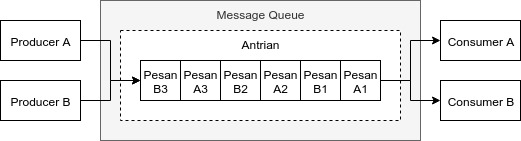
\includegraphics[width=0.75\textwidth]{bab2/img/arsitektur-mq_pnt.jpg}
\caption{Arsitektur Antrian Pesan Push Notification Terpusat}
\label{img:arsitektur-mq_pnt}
\end{figure}
\begin{figure}[H]
	\centering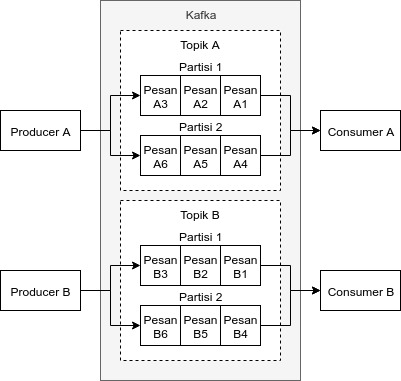
\includegraphics[width=0.75\textwidth]{bab2/img/arsitektur-mq_kafka.jpg}
	\caption{Arsitektur Antrian Pesan Apache Kafka}
	\label{img:arsitektur-mq_kafka}
\end{figure}

\section{Apache Zookeeper}
\par Apache Zookeeper atau Zookeeper adalah layanan tersentralisasi untuk mengatur konfigurasi, penamaan, sinkronisasi sistem terdistribusi, untuk sekelompok layanan \cite{zookeeper-online}.
\par Pada tugas akhir ini, Zookeeper merupakan layanan yang dibutuhkan oleh Kafka untuk beroperasi. Kafka menggunakan Zookeeper untuk mengatur koordinasi \textit{producer} dan \textit{consumer} dengan antrian pesan.

\section{Java}
\par Java adalah bahasa pemrograman yang umum, konkuren, berbasis kelas, dan berbasis objek \cite{java-online}.
\par Pada tugas akhir ini, Java merupakan bahasa pemrograman yang digunakan untuk implementasi Push Notification Terpusat. Alasan pemilihan Java adalah sebagai berikut:
\begin{enumerate}
	\item Mudah untuk dikembangkan
	\item Java didukung penuh oleh pengembang Kafka. Untuk bahasa lain, didukung oleh individu atau tim yang tidak resmi.
	\item Dokumentasi resmi Kafka menggunakan bahasa pemrograman Java.
\end{enumerate}

\section{Spring}
\par Spring adalah sebuah \textit{platform} yang menyediakan dukungan infrastruktur lengkap untuk mengembangkan aplikasi Java \cite{spring-online}. Spring merupakan kerangka kerja yang digunakan untuk mengembangkan Push Notification Terpusat.
\begin{enumerate}
	\item Dukungan pustaka untuk SQL Server dan Kafka.
\end{enumerate}

\section{Actuator}
\par Actuator berisi sekumpulan fitur tambahan untuk pemantauan dan pengaturan aplikasi yang sudah ditahap \textit{production}. Aplikasi bisa dipantau dan diatur dengan menggunakan \textit{endpoint} HTTP atau JMX \cite{actuator-online}.
\par Pada tugas akhir ini, Actuator merupakan pustaka yang digunakan dalam implementasi pemantauan Push Notification Terpusat.

\section{JSON}
\par JSON adalah format pertukaran data yang ringan, berbasis teks, dan independen \cite{json-online}.
\par Pada tugas akhir ini, JSON merupakan format pertukaran data yang digunakan oleh Kafka untuk menyimpan data, dan pustaka Actuator untuk menampilkan \textit{response}.

\section{Docker}
\par Docker adalah \textit{platform} terbuka untuk membangun, mengirim, dan menjalankan aplikasi. Docker memungkinkan pengembang untuk memisahkan kebutuhan infrastruktur dari aplikasi, sehingga proses pengembangan aplikasi bisa lebih cepat \cite{docker-online}.
\par Pada tugas akhir ini, Docker akan digunakan untuk menjalankan Push Notification Terpusat, Kafka, dan Zookeeper. Perbandingan penggunaan Docker dapat dilihat pada Tabel \ref{t:perbandingan_docker}, dan arsitektur Docker pada Gambar \ref{img:arsitektur-docker}.
\begin{longtable}{|p{2.5cm}|p{3.5cm}|p{3.5cm}|}
	\caption{Perbandingan Penggunaan Docker} \label{t:perbandingan_docker} \\ \hline
	\rowcolor{lightgray} & Tanpa Docker & Dengan Docker \\ \hline
	Proses \textit{deployment} & Membutuhkan konfigurasi khusus untuk setiap sistem operasi & Dapat langsung dijalankan di sistem operasi manapun \\ \hline
	Pembatasan sumber daya & Tidak terbatas & Penggunaan CPU dan Memori bisa dibatasi \\ \hline
	Sekuritas & Bergantung pada konfigurasi sistem operasi & \textit{Isolated}, bergantung pada konfigurasi Docker \\ \hline
\end{longtable}
\begin{figure}[H]
\centering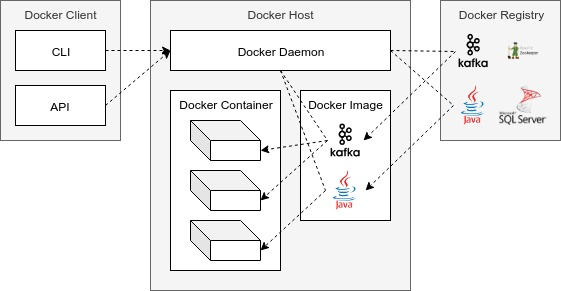
\includegraphics[width=0.75\textwidth]{bab2/img/arsitektur-docker.jpg}
\caption{Arsitektur Docker}
\label{img:arsitektur-docker}
\end{figure}

\section{Docker Compose}
\par Docker Compose adalah alat untuk mendefinisikan dan menjalankan beberapa \textit{container} aplikasi menggunakan Docker. Dengan Docker Compose, pengembang bisa menggunakan file berbasis YAML untuk mengatur konfigurasi layanan aplikasi, dan menggunakannya untuk membuat dan menjalankan layanan aplikasi \cite{docker-compose-online}.
\par Pada tugas akhir ini, Docker Compose akan digunakan untuk mendefinisikan konfigurasi yang digunakan untuk menjalankan Push Notification Terpusat, Kafka, dan Zookeeper. Perbandingan penggunaan Docker Compose dapat dilihat pada Tabel \ref{t:perbandingan_docker_compose}.
\begin{longtable}{|p{2cm}|p{3.5cm}|p{3.5cm}|}
	\caption{Perbandingan Penggunaan Docker Compose} \label{t:perbandingan_docker_compose} \\ \hline
	\rowcolor{lightgray} & Tanpa Compose & Dengan Compose \\ \hline
\end{longtable}

\section{YAML}
\par YAML adalah bahasa untuk serialisasi data yang dirancang agar mudah dipahami oleh manusia dan bisa berjalan dengan bahasa pemrograman modern \cite{yaml-online}.
\par Pada tugas akhir ini, YAML merupakan bahasa yang digunakan oleh Spring dan Docker Compose untuk mendefinisikan konfigurasi yang digunakan untuk menjalankan aplikasi.
